%\documentclass[12pt]{article}

\questionheader{ex:s3.4}


%%%%%%%%%%%%%%%%%%
\subsection*{\Conceptual}
%%%%%%%%%%%%%%%%%%

%%%%%%%%%%%%%%%%%%%%%%%%%%%%
%\Instructions{Questions~\ref{prob_s1.0first} through \ref{prob_s1.0last} provide practice with.}
%%%%%%%%%%%%%%%%%%%%

%%%%%%%%%%%%%%%%%%%%%%%%%%%
\begin{question}
Let $0<\theta<\frac{\pi}{2}$, and $a,b>0$. Denote by $S$ the part of 
the surface $z=y\,\tan\theta$ with $0\le x\le a$, $0\le y\le b$.
\begin{enumerate}[(a)]
\item 
Find the surface area of $S$ without using any calculus.
\item
Find the surface area of $S$ by using Theorem \eref{CLP200}{thm surface area}
in the CLP-3 text.
\end{enumerate}

\end{question}

\begin{hint} 
$S$ is a very simple geometric object.
\end{hint}

\begin{answer} 
$ab\sqrt{1+\tan^2\theta}=ab\sec\theta$
\end{answer}

\begin{solution}
(a) $S$ is the part of the plane $z=y\,\tan\theta$ that lies above the 
rectangle in the $xy$-plane with vertices $(0,0)$, $(a,0)$, $(0,b)$, $(a,b)$. 
So $S$ is the rectangle with vertices $(0,0,0)$, 
$(a,0,0)$, $(0,b,b\tan\theta)$, $(a,b,b\tan\theta)$. So it has side lengths
\begin{align*}
|\llt a,0,0\rgt -\llt 0,0,0\rgt| &=a \\
|\llt 0,b,b\tan\theta\rgt -\llt 0,0,0\rgt| &=  \sqrt{b^2+b^2\tan^2\theta}
\end{align*}
and hence area $ab\sqrt{1+\tan^2\theta}=ab\sec\theta$.

(b) $S$ is the part of the surface $z=f(x,y)$ with $f(x,y) = y\,\tan\theta$
and with $(x,y)$ running over
\begin{equation*}
\cD =\Set{(x,y)}{0\le x\le a,\ 0\le y\le b}
\end{equation*}
Hence by Theorem \eref{CLP200}{thm surface area} in the CLP-3 text
\begin{align*}
\text{Area}(S)&=\dblInt_\cD \sqrt{1+f_x(x,y)^2+f_y(x,y)^2}\ \dee{x}\,\dee{y} \\
&=\int_0^a\dee{x}\int_0^b\dee{y}\ \sqrt{1+0^2+\tan^2\theta} \\
&=ab\sqrt{1+\tan^2\theta}=ab\sec\theta
\end{align*}

\end{solution}



%%%%%%%%%%%%%%%%%%%%%%%%%%%
\begin{question}
Let $c > 0$. Denote by $S$ the part of 
the surface $ax+by+cz=d$ with $(x,y)$ running over the region $D$ in the $xy$-plane.
Find the surface area of $S$, in terms of $a$, $b$, $c$, $d$ and $A(D)$,
the area of the region $D$.
\end{question}

%\begin{hint} 
%\end{hint}

\begin{answer} 
$\frac{\sqrt{a^2+b^2+c^2}}{c} A(D)$
\end{answer}

\begin{solution}
 $S$ is the part of the surface $z=f(x,y)$ with $f(x,y) = \frac{d-ax-by}{c}$
and with $(x,y)$ running over $D$.
Hence by Theorem \eref{CLP200}{thm surface area} in the CLP-3 text
\begin{align*}
\text{Area}(S)&=\dblInt_D \sqrt{1+f_x(x,y)^2+f_y(x,y)^2}\ \dee{x}\,\dee{y} \\
&=\dblInt_D\ \sqrt{1+\frac{a^2}{c^2}+\frac{b^2}{c^2}} \\
&=\frac{\sqrt{a^2+b^2+c^2}}{c} A(D)
\end{align*}

\end{solution}


%%%%%%%%%%%%%%%%%%%%%%%%%%%
\begin{question}
Let $a,b,c > 0$. Denote by $S$ the triangle with vertices $(a,0,0)$,
$(0,b,0)$ and $(0,0,c)$.
\begin{enumerate}[(a)]
\item
Find the surface area of $S$ in three different ways, each using 
Theorem \eref{CLP200}{thm surface area} in the CLP-3 text.
\item
Denote by $T_{xy}$ the projection of $S$ onto the $xy$-plane. (It is the 
triangle with vertices $(0,0,0)$ $(a,0,0)$ and $(0,b,0)$.) Similarly use
$T_{xz}$ to denote the projection of $S$ onto the $xz$-plane and
$T_{yz}$ to denote the projection of $S$ onto the $yz$-plane. Show that
\begin{equation*}
\text{Area}(S) =\sqrt{\text{Area}(T_{xy})^2
                     +\text{Area}(T_{xz})^2
                     +\text{Area}(T_{yz})^2
                     }
\end{equation*}

\end{enumerate}
\end{question}

\begin{hint} 
The triangle is part of the plane $\frac{x}{a}+\frac{y}{b} +\frac{z}{c}=1$.
\end{hint}

\begin{answer} 
(a) $\frac{1}{2}\sqrt{a^2b^2+a^2c^2+b^2c^2}$

(b) See the solution.
\end{answer}

\begin{solution}
Note that all three vertices $(a,0,0)$, $(0,b,0)$ and $(0,0,c)$ lie on 
the plane $\frac{x}{a}+\frac{y}{b} +\frac{z}{c}=1$. So the triangle is 
part of that plane.

\emph{Method 1.}\ \ \ 
 $S$ is the part of the surface $z=f(x,y)$ with 
$f(x,y) = c\left(1-\frac{x}{a}-\frac{y}{b}\right)$
and with $(x,y)$ running over the triangle $T_{xy}$ in the $xy$-plane 
with vertices $(0,0,0)$ $(a,0,0)$ and $(0,b,0)$.
Hence by part a of Theorem \eref{CLP200}{thm surface area} in the CLP-3 text
\begin{align*}
\text{Area}(S)&=\dblInt_{T_{xy}} \sqrt{1+f_x(x,y)^2+f_y(x,y)^2}\ \dee{x}\,\dee{y} \\
&=\dblInt_{T_{xy}}\ \sqrt{1+\frac{c^2}{a^2}+\frac{c^2}{b^2}}\  
\dee{x}\,\dee{y} \\
&=\sqrt{1+\frac{c^2}{a^2}+\frac{c^2}{b^2}}\ A(T_{xy})
\end{align*}
where $A(T_{xy})$ is the area of $T_{xy}$. Since the triangle $T_{xy}$ 
has base $a$ and height $b$ (see the figure below), it has 
area $\frac{1}{2}ab$. So
\begin{equation*}
\text{Area}(S)=\frac{1}{2}\sqrt{1+\frac{c^2}{a^2}+\frac{c^2}{b^2}}\ ab 
 =\frac{1}{2}\sqrt{a^2b^2+a^2c^2+b^2c^2}
\end{equation*}

\begin{center}
     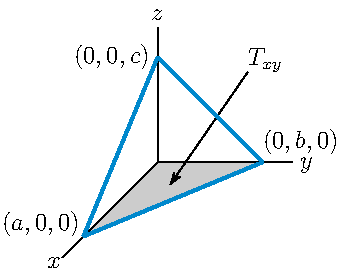
\includegraphics{triangleProjection.pdf}
\end{center}


\emph{Method 2.}\ \ \ 
 $S$ is the part of the surface $x=g(y,z)$ with 
$g(y,z) = a\left(1-\frac{y}{b}-\frac{z}{c}\right)$
and with $(y,z)$ running over the triangle $T_{yz}$ in the $yz$-plane 
with vertices $(0,0,0)$ $(0,b,0)$ and $(0,0,c)$.
Hence by part b of Theorem \eref{CLP200}{thm surface area} in the CLP-3 text
\begin{align*}
\text{Area}(S)&=\dblInt_{T_{yz}} \sqrt{1+g_y(y,z)^2+g_z(y,z)^2}\ \dee{y}\,\dee{z} \\
&=\dblInt_{T_{yz}}\ \sqrt{1+\frac{a^2}{b^2}+\frac{a^2}{c^2}}\  
\dee{y}\,\dee{z}\\
&=\sqrt{1+\frac{a^2}{b^2}+\frac{a^2}{c^2}}\ A(T_{yz})
\end{align*}
where $A(T_{yz})$ is the area of $T_{yz}$. Since $T_{yz}$ has base $b$ and 
height $c$, it has area $\frac{1}{2}bc$. So
\begin{equation*}
\text{Area}(S)=\frac{1}{2}\sqrt{1+\frac{a^2}{b^2}+\frac{a^2}{c^2}}\ bc 
 =\frac{1}{2}\sqrt{a^2b^2+a^2c^2+b^2c^2}
\end{equation*}

\emph{Method 3.}\ \ \ 
 $S$ is the part of the surface $y=h(x,z)$ with 
$h(x,z) = b\left(1-\frac{x}{a}-\frac{z}{c}\right)$
and with $(x,z)$ running over the triangle $T_{xz}$ in the $xz$-plane 
with vertices $(0,0,0)$ $(a,0,0)$ and $(0,0,c)$.
Hence by part c of Theorem \eref{CLP200}{thm surface area} in the CLP-3 text
\begin{align*}
\text{Area}(S)&=\dblInt_{T_{xz}} \sqrt{1+h_x(x,z)^2+h_z(x,z)^2}\ \dee{x}\,\dee{z} \\
&=\dblInt_{T_{xz}}\ \sqrt{1+\frac{b^2}{a^2}+\frac{b^2}{c^2}}\  
\dee{x}\,\dee{z}\\
&=\sqrt{1+\frac{b^2}{a^2}+\frac{b^2}{c^2}}\ A(T_{xz})
\end{align*}
where $A(T_{xz})$ is the area of $T_{xz}$. Since $T_{xz}$ has base $a$ and 
height $c$, it has area $\frac{1}{2}ac$. So
\begin{equation*}
\text{Area}(S)=\frac{1}{2}\sqrt{1+\frac{b^2}{a^2}+\frac{b^2}{c^2}}\ bc 
 =\frac{1}{2}\sqrt{a^2b^2+a^2c^2+b^2c^2}
\end{equation*}

(b) We have already seen in the solution to part (a) that
\begin{equation*}
\text{Area}(T_{xy})=\frac{ab}{2}\qquad
\text{Area}(T_{xz})=\frac{ac}{2}\qquad
\text{Area}(T_{yz})=\frac{bc}{2}\qquad
\end{equation*}
Hence
\begin{align*}
\text{Area}(S) 
&=\sqrt{\frac{a^2b^2}{4}+\frac{a^2c^2}{4}+\frac{b^2c^2}{4}} \\
&=\sqrt{\text{Area}(T_{xy})^2
                     +\text{Area}(T_{xz})^2
                     +\text{Area}(T_{yz})^2
                     }
\end{align*}

\end{solution}


%%%%%%%%%%%%%%%%%%
\subsection*{\Procedural}
%%%%%%%%%%%%%%%%%%

%%%%%%%%%%%%%%%%%%%%%%%%%%%
\begin{question}[M317 2002A] %3
 Find the area of the part of the surface $z=y^{3/2}$ that
lies above $0\le x,y\le 1$.
\end{question}

%\begin{hint} 
%\end{hint}

\begin{answer} 
$\frac{8}{27}\left[\left(\frac{13}{4}\right)^{3/2}-1\right]$
\end{answer}


\begin{solution}
For the surface $z=f(x,y)=y^{3/2}$,
\begin{equation*}
\dee{S}=\sqrt{1+f_x^2+f_y^2}\ \dee{x}\dee{y}
=\sqrt{1+\Big(\frac{3}{2}\sqrt{y}\Big)^2}\ \dee{x}\dee{y}
=\sqrt{1+\frac{9}{4}y}\ \dee{x}\dee{y}
\end{equation*}
by Theorem \eref{CLP200}{thm surface area}.a in the CLP-3 text,
So the area is
\begin{align*}
\int_0^1\dee{x}\int_0^1\dee{y}\ \sqrt{1+\frac{9}{4}y}
&=\int_0^1\dee{x}\ \frac{8}{27}\Big[\Big(1+\frac{9}{4}y\Big)^{3/2}\Big]_0^1
=\int_0^1\dee{x}\ \frac{8}{27}\Big[\Big(\frac{13}{4}\Big)^{3/2}-1\Big] \\
&=\frac{8}{27}\left[\left(\frac{13}{4}\right)^{3/2}-1\right]
\end{align*}
\end{solution}


%%%%%%%%%%%%%%%%%%%%%%%%%%%%%%%%
\begin{question}[M253 2013D] %4
Find the surface area of the part of the paraboloid 
$z = a^2 - x^2 - y^2$ which lies above the $xy$--plane.
\end{question}

%\begin{hint}
%\end{hint}

\begin{answer}
$\frac{\pi}{6}\big[{(1+4a^2)}^{3/2}-1\big]$
\end{answer}

\begin{solution}
First observe that any point $(x,y,z)$ on the paraboliod lies above the $xy$-plane if and only if
\begin{equation*}
0\le z = a^2-x^2-y^2
\iff x^2+y^2\le a^2
\end{equation*} 
That is, if and only if $(x,y)$ lies in the circular disk of radius $a$
centred on the origin. The equation of the paraboloid is of the form 
$z=f(x,y)$ with $f(x,y)=a^2-x^2-y^2$. So, by 
Theorem \eref{CLP200}{thm surface area}.a in the CLP-3 text,
\begin{align*}
\text{Surface area}
&= \dblInt_{x^2+y^2\le a^2}\sqrt{1+f_x(x,y)^2+f_y(x,y)^2}\ \dee{x}\,\dee{y} \\
&= \dblInt_{x^2+y^2\le a^2}\sqrt{1+4x^2+4y^2}\ \dee{x}\,\dee{y}
\end{align*}
Switching to polar coordinates,
\begin{align*}
\text{Surface area}
&= \int_0^a\dee{r}\int_0^{2\pi}\dee{\theta}\ r\sqrt{1+4r^2}\\
&= 2\pi \int_0^a\dee{r}\ r\sqrt{1+4r^2}\\
&= 2\pi \int_1^{1+4a^2}\frac{\dee{s}}{8}\ \sqrt{s}\qquad
\text{with $s=1+4r^2$, $\dee{s}=8r\,\dee{r}$} \\
&=\frac{\pi}{4}\ \frac{2}{3}s^{3/2}\bigg|_{s=1}^{s=1+4a^2} \\
&=\frac{\pi}{6}\big[{(1+4a^2)}^{3/2}-1\big]
\end{align*}

\end{solution}


%%%%%%%%%%%%%%%%%%%%%%%%%%%%%%%%
\begin{question}[M253 2014D] %7a
Find the area of the portion of the cone $z^2 = x^2 + y^2$ 
lying between the planes $z = 2$ and $z = 3$.
\end{question}

%\begin{hint}
%\end{hint}

\begin{answer}
$5\sqrt{2}\pi$
\end{answer}

\begin{solution}
First observe that any point $(x,y,z)$ on the cone lies between the 
planes $z=2$ and $z=3$ if and only if $4\le x^2+y^2\le 9$.
%That is, if and only if $(x,y)$ has polar coordinate $r$ between $2$ and $3$. 
The equation of the cone can be rewritten in the form 
$z=f(x,y)$ with $f(x,y)=\sqrt{x^2+y^2}$. Note that
\begin{align*}
f_x(x,y)=\frac{x}{\sqrt{x^2+y^2}}\qquad
f_y(x,y)=\frac{y}{\sqrt{x^2+y^2}}
\end{align*}
So, by 
Theorem \eref{CLP200}{thm surface area}.a in the CLP-3 text,
\begin{align*}
\text{Surface area}
&= \dblInt_{4\le x^2+y^2\le 9}\sqrt{1+f_x(x,y)^2+f_y(x,y)^2}\ \dee{x}\,\dee{y} \\
&= \dblInt_{4\le x^2+y^2\le 9}
    \sqrt{1+\frac{x^2}{x^2+y^2}+\frac{y^2}{x^2+y^2}}\ \dee{x}\,\dee{y} \\
&=\sqrt{2} \dblInt_{4\le x^2+y^2\le 9} \dee{x}\,\dee{y} 
\end{align*}
Now the domain of integration is a circular washer with outside radius $3$
and inside radius $2$ and hence of area $\pi(3^2-2^2)=5\pi$. So the surface area is $5\sqrt{2}\pi$.

\end{solution}
%%%%%%%%%%%%%%%%%%%%%%%%%%%%%%%%
\begin{question}[M253 2015D] %8
Determine the surface area of the surface given by 
$z = \frac{2}{3}\big(x^{3/2} + y^{3/2}\big)$, over the square
$0 \le  x \le  1$, $0 \le  y \le  1$.
\end{question}

%\begin{hint}
%\end{hint}

\begin{answer}
$\frac{4}{15}\big[9\sqrt{3}-8\sqrt{2}+1\big]$
\end{answer}

\begin{solution}
The equation of the surface is of the form 
$z=f(x,y)$ with $f(x,y)=\frac{2}{3}\big(x^{3/2} + y^{3/2}\big)$. Note that
\begin{align*}
f_x(x,y)=\sqrt{x}\qquad
f_y(x,y)=\sqrt{y}
\end{align*}
So, by Theorem \eref{CLP200}{thm surface area}.a in the CLP-3 text,
\begin{align*}
\text{Surface area}
&= \int_0^1\dee{x}\int_0^1\dee{y}\ \sqrt{1+f_x(x,y)^2+f_y(x,y)^2} \\
&= \int_0^1\dee{x}\int_0^1\dee{y}\ \sqrt{1+x+y} \\
&= \int_0^1\dee{x}\ \Big[\frac{2}{3}(1+x+y)^{3/2}\Big]_{y=0}^{y=1} \\
&= \frac{2}{3}\int_0^1\dee{x}\ \big[(2+x)^{3/2}-(1+x)^{3/2}\big] \\
&= \frac{2}{3}\ \frac{2}{5}\Big[(2+x)^{5/2}-(1+x)^{5/2}\Big]_{x=0}^{x=1} \\
&= \frac{4}{15} \big[3^{5/2}-2^{5/2}-2^{5/2}+1^{5/2}\big] \\
&= \frac{4}{15}\big[9\sqrt{3}-8\sqrt{2}+1\big]
\end{align*}
\end{solution}

%%%%%%%%%%%%%%%%%%%%%%%%%%%%%%%%
\begin{question}[M253 2016D] %2
\begin{enumerate}[(a)]
\item
To find the surface area of the surface $z = f (x,y)$ above the region $D$, 
we integrate $\dblInt_D F(x,y)\ \dee{A}$. What is $F(x,y)$?
\item
Consider a ``Death Star'',  a ball of radius $2$ centred at the origin 
with another ball of radius $2$ centred at $(0, 0, 2\sqrt{3})$ cut out of it. 
The diagram below shows the slice where $y = 0$.

\begin{center}
     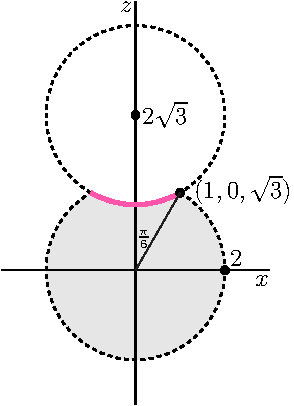
\includegraphics{OE253_16D_2.pdf}
\end{center}

\begin{enumerate}[(i)]
\item
The Rebels want to paint part of the surface of Death Star hot pink; specifically, the concave part (indicated with a thick line in the diagram). 
To help them determine how much paint is needed, carefully fill in the 
missing parts of this integral:
\begin{equation*}
\text{surface area} = 
\int_{\underline{\ \ \ \ }}^{\underline{\ \ \ \ }}
                 \int_{\underline{\ \ \ \ }}^{\underline{\ \ \ \ }}
                        \underline{\ \ \ \ \ \ \ \ \ \ }\ \dee{r}\,\dee{\theta}
\end{equation*}

\item
What is the total surface area of the Death Star?
\end{enumerate}
\end{enumerate}
\end{question}

\begin{hint}
The total surface area of (b) (ii) can be determined without evaluating
any integrals.
\end{hint}

\begin{answer}
(a)  $F(x,y) = \sqrt{1+f_x(x,y)^2+f_y(x,y)^2}$
\qquad
(b) (i) $\int_0^{2\pi}\dee{\theta}\int_0^1\dee{r}\ \frac{2r}{\sqrt{4-r^2}}$ 
\qquad (ii) $16\pi$
\end{answer}

\begin{solution}
(a)
By Theorem \eref{CLP200}{thm surface area}.a in the CLP-3 text,
$F(x,y) = \sqrt{1+f_x(x,y)^2+f_y(x,y)^2}$.

(b)  (i) The ``dimple'' to be painted is part of the upper sphere
$x^2+y^2+\big(z-2\sqrt{3}\big)^2=4$. It is on the bottom half of the sphere
and so has equation $z=f(x,y)=2\sqrt{3}-\sqrt{4-x^2-y^2}$. Note that
\begin{align*}
f_x(x,y) = \frac{x}{\sqrt{4-x^2-y^2}}\qquad
f_y(x,y) = \frac{y}{\sqrt{4-x^2-y^2}}
\end{align*}
The point on the dimple with the largest value of $x$ is
$(1,0,\sqrt{3})$. (It is marked by a dot in the figure above.) The dimple
is invariant under rotations around the $z$--axis and so has $(x,y)$
running over $x^2+y^2\le 1$. So, by 
Theorem \eref{CLP200}{thm surface area}.a in the CLP-3 text,
\begin{align*}
\text{Surface area}
&= \dblInt_{x^2+y^2\le 1}\sqrt{1+f_x(x,y)^2+f_y(x,y)^2}\ \dee{x}\,\dee{y} \\
&= \dblInt_{x^2+y^2\le 1}\sqrt{1+\frac{x^2}{4-x^2-y^2}
                                +\frac{y^2}{4-x^2-y^2}}\ \dee{x}\,\dee{y} \\
&= \dblInt_{x^2+y^2\le 1}\frac{2}{\sqrt{4-x^2-y^2}}\ \dee{x}\,\dee{y} 
\end{align*}
Switching to polar coordinates,
\begin{align*}
\text{Surface area}
&= \int_0^{2\pi}\dee{\theta}\int_0^1\dee{r}\ \frac{2r}{\sqrt{4-r^2}}
\end{align*}

(b) (ii) Observe that if we flip the dimple up by reflecting it
in the plane $z=\sqrt{3}$, as in the figure below, the ``Death Star'' 
becomes a perfect ball of radius $2$.  
\begin{center}
     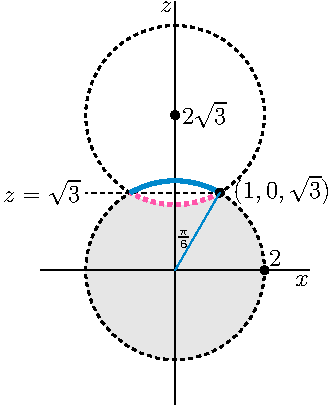
\includegraphics{OE253_16D_2a.pdf}
\end{center}
The area of the pink dimple in the figure above is identical to the area
of the blue cap in that figure. So the total surface area of the 
Death Star is exactly the surface area of a sphere of radius $a=2$ and so
(see Example \eref{CLP200}{eg area hemisphere} in the CLP-3 text)
is $4\pi a^2 = 4 \pi 2^2=16\pi$.

\end{solution}

%%%%%%%%%%%%%%%%%%%%%%%%%%%%%%%%%%%%%%%%%
\begin{question} [M200 2003A] % 7b
Find the area of the cone $z^2=x^2+y^2$ between $z=1$ and $z=16$.
\end{question}

%\begin{hint}
%
%\end{hint}

\begin{answer}
$255\sqrt{2}\pi\approx 1132.9$
\end{answer}

\begin{solution}
On the upper half of the cone 
\begin{equation*}
z=f(x,y)=\sqrt{x^2+y^2}\qquad 
f_x(x,y)=\frac{x}{\sqrt{x^2+y^2}}\qquad
f_y(x,y)=\frac{y}{\sqrt{x^2+y^2}}
\end{equation*}
so that
\begin{equation*}
\dee{S}=\sqrt{1+f_x(x,y)^2+f_y(x,y)^2}\,\dee{x}\,\dee{y}
=\sqrt{1+\frac{x^2}{x^2+y^2}+\frac{y^2}{x^2+y^2}}\,\dee{x}\,\dee{y}
=\sqrt{2}\,\dee{x}\,\dee{y}
\end{equation*}
and
\begin{align*}
\text{Area}&= \dblInt_{1\le x^2+y^2\le 16^2}\sqrt{2}\,\dee{x}\,\dee{y} \\
&=\sqrt{2}\,\Big[\text{area of }\Set{(x,y)}{x^2+y^2\le 16^2}-
           \text{area of }\Set{(x,y)}{x^2+y^2\le 1}\Big] \\
&=\sqrt{2}\,\big[\pi 16^2-\pi 1^2\big]
=255\sqrt{2}\pi\approx 1132.9
\end{align*}
\end{solution}

%%%%%%%%%%%%%%%%%%%%%%%%%%%%%%%%%%%%%%%%%
\begin{question} [M200 2001D] %7
Find the surface area of that part of the hemisphere 
$z=\sqrt{a^2-x^2-y^2}$ which lies within the cylinder $\big(x-\frac{a}{2}\big)^2+y^2=\big(\frac{a}{2}\big)^2$.
\end{question}

%\begin{hint}
%
%\end{hint}

\begin{answer}
$a^2[\pi-2]$
\end{answer}

\begin{solution}
We are to find the surface area of part of a hemisphere. On the hemisphere 
\begin{align*}
z=f(x,y)=\sqrt{a^2-x^2-y^2}\qquad 
f_x(x,y)=-\frac{x}{\sqrt{a^2-x^2-y^2}}\qquad
f_y(x,y)=-\frac{y}{\sqrt{a^2-x^2-y^2}}
\end{align*}
so that
\begin{align*}
\dee{S}&=\sqrt{1+f_x(x,y)^2+f_y(x,y)^2}\,\dee{x}\,\dee{y}
=\sqrt{1+\frac{x^2}{a^2-x^2-y^2}+\frac{y^2}{a^2-x^2-y^2}}\,\dee{x}\,\dee{y} \\
&=\sqrt{\frac{a^2}{a^2-x^2-y^2}}\,\dee{x}\,\dee{y}
\end{align*}
In polar coordinates, this is $\dee{S}=\frac{a}{\sqrt{a^2-r^2}}\,r\,\dee{r}\,\dee{\theta}$.
We are to find the surface area of the part of the hemisphere that is 
inside the cylinder, $x^2-ax+y^2=0$, which is polar coordinates is
becomes $r^2-ar\cos\theta=0$ or $r=a\cos\theta$. The top half of the domain of
integration is sketched below.  
\begin{center}
     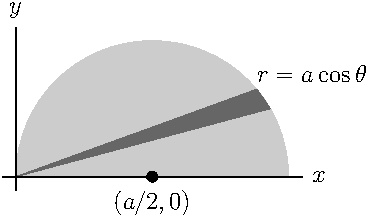
\includegraphics{OE01DQ7.pdf}
\end{center}
So the
\begin{align*}
{\rm Surface\ Area}
&= 2\int_0^{\pi/2}\dee{\theta}\int_0^{a\cos\theta}\dee{r}\ r
                                      \frac{a}{\sqrt{a^2-r^2}}
= 2a\int_0^{\pi/2}\dee{\theta}\ \Big[-\sqrt{a^2-r^2}\,\Big]_0^{a\cos\theta}
\\
&= 2a\int_0^{\pi/2}\dee{\theta}\ \big[a-a\sin\theta\big] \\
&= 2a^2\Big[\theta+\cos\theta\Big]_0^{\pi/2}
=a^2[\pi-2]
\end{align*}
\end{solution}




%%%%%%%%%%%%%%%%%%
%\subsection*{\Application}
%%%%%%%%%%%%%%%%%%
